\documentclass[prb,12pt]{revtex4-2}

\usepackage{amsmath, amssymb,physics,amsfonts,amsthm}
\usepackage{enumitem}
\usepackage{cancel}
\usepackage{booktabs}
\usepackage{tikz}
\usepackage{hyperref}
\usepackage{enumitem}
\usepackage{transparent}
\usepackage{float}
\usepackage{multirow}
\newtheorem{Theorem}{Theorem}
\newtheorem{Proposition}{Theorem}
\newtheorem{Lemma}[Theorem]{Lemma}
\newtheorem{Corollary}[Theorem]{Corollary}
\newtheorem{Example}[Theorem]{Example}
\newtheorem{Remark}[Theorem]{Remark}
\theoremstyle{definition}
\newtheorem{Problem}{Problem}
\theoremstyle{definition}
\newtheorem{Definition}[Theorem]{Definition}
\newenvironment{parts}{\begin{enumerate}[label=(\alph*)]}{\end{enumerate}}
%tikz
\usetikzlibrary{patterns}
% definitions of number sets
\newcommand{\N}{\mathbb{N}}
\newcommand{\R}{\mathbb{R}}
\newcommand{\Z}{\mathbb{Z}}
\newcommand{\Q}{\mathbb{Q}}
\newcommand{\C}{\mathbb{C}}
\begin{document}
	\title{Einf\"{u}rung in die Algebra Hausaufgaben Blatt Nr. 1}
	\author{Jun Wei Tan}
	\email{jun-wei.tan@stud-mail.uni-wuerzburg.de}
	\affiliation{Julius-Maximilians-Universit\"{a}t W\"{u}rzburg}
	\date{\today}
	\maketitle
%\begin{Problem}
	\begin{parts}
		\item Geben Sie die Definitionen von Gradient, Rotation und Divergenz an.
		\item Wir schreiben die Komponenten des dreidimensionalen Vektorprodukts als
			\[
				(\vec{a}\times \vec{b})_i=\sum_{j,k=1}^3 \epsilon_{ijk}a_jb_k,\] 
				wobei $\epsilon_{ijk}$ der total antisymmetrische Tensor f\"{u}r $\R^3$ ist, mit $\epsilon_{ijk}=1$. Zeigen Sie, dass gilt:
				\begin{align*}
					\sum_{i=1}^3 \epsilon_{ijk}\epsilon_{ilm}=&\delta_{jl}\delta_{km}-\delta_{jm}\delta_{kl}\\
					\frac{1}{2}\sum_{i,j=1}^3 \epsilon_{ijk}\epsilon_{jl}\delta_{kl},
				\end{align*}
				mit $\delta$ dem Kronecker-$\delta$.
			\item Zeigen Sie mit den Formeln aus (b) die folgenden Identitäten für beliebige Vektorfelder $\vec{a},~\vec{b},~\vec{c},~\vec{d}$:
				\begin{align*}
					\vec{a}\cdot(\vec{b}\times\vec{c})&=\vec{b}\cdot (\vec{c}\times \vec{a})=\vec{c}\cdot (\vec{a}\times \vec{b})\\
					\vec{a}\times(\vec{b}\times\vec{c})=&(\vec{a}\cdot\vec{c})\vec{b}-(\vec{a}\cdot\vec{b})\vec{c},\\
					(\vec{a}\times\vec{b})\cdot(\vec{c}\times\vec{d})=*(\vec{a}\cdot\vec{c})(\vec{b}\cdot\vec{d})-(\vec{a}\cdot\vec{d})(\vec{b}\cdot\vec{c})
				\end{align*}
			\item Zeigen Sie damit, dass f\"{u}r beliebige skalare Funktionen $F(\vec{x})$ und Vektorfelder $\vec{A}(\vec{x})$ gilt:
				\begin{align*}
					\curl{\grad{F}}=&0\\
					\div{(\curl{A})}=&0\\
					\curl{\curl{A}}=&\grad{(\div{A})}-\laplacian{A}\\
					\div{(F\vec{A})}=(\grad{F})\cdot\vec{A}+F\div{\vec{A}},
				\end{align*}
				mit $\Delta$ dem Laplace-Operator.
	\end{parts}
\end{Problem} 
\begin{proof}
	\begin{parts}
	\item 
		\begin{align*}
			\text{grad }F=\sum_{i=1}^3 \pdv{F}{x_i}\hat{x}_i\\
			\text{div }\vec{F}=\sum_{i=1}^3 \pdv{F_i}{x_i}\\
			\text{curl }\vec{F}=&\ldots
		\end{align*}
	\item Offensichtlich muss $j\neq k$ und $l\neq m$ sein, ansonsten wäre 1
	\end{parts}
\end{proof}
\begin{Problem}
	
\end{Problem}

\begin{Problem}
	Betrachten Sie die folgenden Familien von Kraftfeldern auf geeigneten Definitionsbereichen $D_\eta^{(n)}  \subseteq \R^3$
	\begin{align*}
		F_\eta^{(1)}:& D_\eta^{(1)}\ni \va x\to r^\eta\cdot \va x\in \R^3\\
		F_\eta^{(2)}:& D_\eta^{(2)}\ni\va x \to r_{12}^\eta\cdot(x_1\va e_1-x_2\va e_2)\in \R^3\\
		F_\eta^{(3)}:& D_\eta^{(3)}\ni \va x\to r_{12}^\eta\cdot\left( x_2\va e_1-x_1\va e_2 \right) \in\R^3\\
		F_\eta^{(4)}:&D_\eta^{(3)}\ni \va x\to r_{12}^\eta\cdot\left( x_2\va e_1+x_1\va e_2 \right) \in \R^3
	\end{align*}
	wobei $r_{12}=\sqrt{x_1^2+x_2^2} $ und $r=\sqrt{x_1^2+x_2^2+x_3^3} $
	Skizzieren Sie die Felder $\va F_\eta^{(n)}$ als Vektorpfeile in der von den Einheitsvektoren $\va e_1$ und $\va e_2$ aufgespannten Ebene (hier genügt es, zwischen den Fällen $\eta > -1, \eta = -1$ und $\eta < -1$ zu unterscheiden). 
	
	Bestimmen Sie, abhängig von der Potenz $\eta \in \R$,
	\begin{enumerate}
		\item den maximalen Definitionsbereich $D_\eta^{(n)}$,
		\item die maximale Bereiche $C_\eta^{(n)}\subseteq D_\eta^{(n)}$, auf denen $F_\eta^{(n)}$ konservativ ist,
		\item eine Potentialfunktion $V_\eta^{(n)}:C_{\eta}^{(n)}\to \R$ mit $F_\eta^{(n)}=-\grad{V_\eta^{(n)}}$, sofern sie existiert,
		\item das Kurvenintegral
		\[I_\eta^{(n)}(R)=\int_{\gamma_R}\dd{\va\xi}\cdot\va F_\eta^{(n)}(\va\xi)\]
		über den gegen den Uhrzeigersinn umlaufenen Kreis $\gamma_R$ mit Radius $R$ und Mittelpunkt $\va0$ in der von $\va e_1$ und $\va e_2$ aufgespannten Ebene
		\begin{center}
			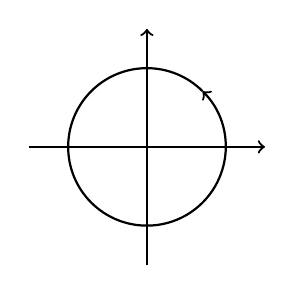
\begin{tikzpicture}
				\draw[thick, ->] (-1.5,0) -- (1.5,0);
				\draw[thick, ->] (0,-1.5) -- (0,1.5);
				\draw[thick, ->] ({1/sqrt(2)},{1/sqrt(2)}) arc (45:405:1);
			\end{tikzpicture}
		\end{center}
	\end{enumerate}
\end{Problem}

\end{document}
